\section{Mehrprozessorsysteme}

\begin{defi}{Flynnsche Klassifikation}
    % https://de.wikipedia.org/wiki/Flynnsche_Klassifikation (Quelle)
    Die \emph{flynnsche Klassifikation}  ist eine Unterteilung von Rechnerarchitekturen, welche 1966 von Michael J. Flynn publiziert wurde.
    Dabei werden die Architekturen nach der Anzahl der vorhandenen Befehls- (Instruction Streams) und Datenströme (Data Streams) unterteilt.

    Die vier Kategorien sind:
    \begin{itemize}
        \item \emph{SISD}: Single Instruction, Single Data
        \begin{itemize}
            \item nicht parallel
            \item z. B. Von-Neumann-Rechner
        \end{itemize}
        \item \emph{SIMD}: Single Instruction, Multiple Data
        \begin{itemize}
            \item z. B. Vektor- oder Arrayprozessoren
        \end{itemize}
        \item \emph{MISD}: Multiple Instruction, Single Data
        \begin{itemize}
            \item irrelevant
        \end{itemize}
        \item \emph{MIMD}: Multiple Instruction, Multiple Data
        \begin{itemize}
            \item speichergekoppelte Multiprozessoren (Shared Memory)
            \item nachrichtengekoppelte Multiprozessoren
        \end{itemize}
    \end{itemize}

    \centering
    % TODO: https://en.wikipedia.org/wiki/Flynn%27s_taxonomy (Quelle)
    \begin{tabular}{cc}
    \end{tabular}
\end{defi}

\begin{bonus}[Flynn'sche Klassifikation]{Erweiterungen}
    \begin{center}
        \begin{forest}
            for tree={inner sep=2pt,outer sep=0pt,align=center,font=\sffamily\footnotesize,draw}
            [Parallelrechner
            [\emph{SIMD} \\ Single \\ Instruction \\ Multiple \\ Data
            [Vektor- \\ Prozessoren \\ (auch Mischformen \\ mit MIMD vorhanden!)]
            [Array- \\ Prozessoren]
            ]
            [\emph{MIMD} \\ Multiple \\ Instruction \\ Multiple \\ Data
            [Speichergekoppelte \\ Multiprozessoren
            [Unified \\ Memory \\ Architecture \\ (UMA)]
            [Non-Uniform \\ Memory \\ Access \\ (NUMA)]
            ]
            [Nachrichtengekoppelte \\ Multiprozessoren
            [Massively \\ Parallel \\ Processing \\ (MPP)]
            [Cluster Of \\ Workstations \\ (COW)]
            ]
            ]
            ]
        \end{forest}
    \end{center}
\end{bonus}
\begin{defi}{Shared Memory}
    % TODO: https://de.wikipedia.org/wiki/Shared_Memory (Quelle)
    Bei MIMD-Architekturen unterscheidet man eng gekoppelte und lose gekoppelte Systeme, wobei Mehrprozessorsysteme zur Klasse der eng gekoppelten Systeme gehören.
    In eng gekoppelten Mehrprozessorsystemen teilen sich die verschiedenen Prozessoren einen gemeinsamen Speicher (\emph{Shared Memory}).

    Gegenüber lose gekoppelten MIMD-Architekturen hat dies folgende Vorteile:
    \begin{itemize}
        \item die Prozessoren haben alle dieselbe Sicht auf die Daten und können daher auf einfache Art und Weise miteinander kommunizieren
        \item der Zugriff auf den gemeinsamen Speicher erfolgt sehr schnell
    \end{itemize}

    Aus diesen Gründen ist ein eng gekoppeltes MIMD-System in der Regel einfacher zu programmieren als ein lose gekoppeltes MIMD-System.

    Allerdings kann der gemeinsam genutzte Speicher auch schnell zum Flaschenhals werden, wenn zu viele Prozessoren vorhanden sind, da (bei einem gemeinsam genutzten Speicherbus) zu einer Zeit immer nur ein Prozessor auf den Speicher zugreifen kann.
    \begin{defi}{Speichergekoppelte Systeme}
        Bei speichergekoppelten Multiprozessoren arbeiten alle Prozessoren in einem einheitlichen Adressraum.

        Je nach physiklischer Speicherorganisation unterscheidet man:
        \begin{itemize}
            \item Symmetrische Multiprozessoren (SMP, symmetric multiprocessor),
            bei denen gleichartige Prozessoren über ein Verbindungsnetzwerk mit einem gemeinsamen Speicher verbunden sind
            \item Distributed-Shared-Memory Systeme,
            bei denen zwar ein einheitlicher Adressraum existiert,
            aber die Speicher physikalisch auf einzelnen Verarbeitungsknoten verteilt sind
        \end{itemize}

        \emph{Bemerkungen:}
        \begin{itemize}
            \item Speichergekoppelte Multiprozessoren gelten als einfacher programmierbar gegenüber nachrichtengekoppelten Multiprozessoren
            \item Nutzbare Parallelität reicht von der Programmebene bis zur Blockebene
            \item Autoparallelisierende Compiler nutzen insbesondere die Parallelisierung der Schleifenebene (einzelne Iterationen nebenläufig abarbeitbar)
        \end{itemize}
    \end{defi}

    \begin{defi}[Shared Memory]{Uniform Memory Access}
        % TODO: https://de.wikipedia.org/wiki/Uniform_Memory_Access (Quelle)
        \emph{Uniform Memory Access} (\emph{UMA}) steht allgemein für eine Speicherarchitektur in Mehrprozessorsystemen.
        Dabei gibt es nur einen globalen Speicher, auf den von allen Prozessoren aus einheitlich zugegriffen werden kann.
        Im Idealfall jeweils mit derselben Bandbreite und Latenzzeit, weshalb solch ein System auch \emph{Symmetrisches Multiprozessorsystem} (\emph{SMP}) genannt wird.

        Das Konzept steht im Gegensatz zu NUMA, bei dem die Zugriffszeit auf den Speicher vom Ort des Speichers abhängen.

        TODO: Grafik
    \end{defi}

    \begin{defi}[Shared Memory]{Non-Uniform Memory Access}
        % TODO: https://de.wikipedia.org/wiki/Non-Uniform_Memory_Access (Quelle)
        \emph{Non-Uniform Memory Access} (\emph{NUMA}) ist eine Computer-Arbeitsspeicher-Architektur für Multiprozessorsysteme, bei denen jeder Prozessor einen eigenen, \enquote{lokalen} Arbeitsspeicher hat, aber anderen Prozessoren über einen gemeinsamen Adressraum \enquote{direkten} Zugriff darauf gewährt (\emph{Distributed Shared Memory}).

        Die Speicherzugriffszeiten für eine CPU in einem solchen Verbund hängen daher davon ab, ob sich eine Speicheradresse im CPU-eigenen \enquote{lokalen} oder im \enquote{fremden} Speicher (einer anderen CPU) befindet.

        TODO: Grafik
    \end{defi}

    \begin{defi}{Nachrichtengekoppelte Systeme}
        % TODO: https://pc2.uni-paderborn.de/fileadmin/pc2/lecture_APRS19/VL_APCS.03.pdf (Quelle)
        Beim \emph{nachrichtengekoppelten Multiprozessorsystem} besitzen alle Prozessoren nur räumlich verteilte Speicher und prozessorlokale Adressräume.

        Die Kommunikation geschieht durch Austausch von Nachrichten.

        TODO: Grafik
    \end{defi}

    \subsection{Verbindungsnetzwerke}

    \begin{defi}{Verbindungsnetzwerk}
        % TODO: https://de.wikipedia.org/wiki/Verbindungsnetzwerk (Quelle)
        Das \emph{Verbindungsnetzwerk} ermöglicht den Datenaustausch und die Verteilung des Programms zwischen den Prozessoren.

        Um einen hohen Datentransfer zu erhalten, wird eine große Anzahl von physischen Verbindungen benötigt.
    \end{defi}

    \begin{defi}[Verbindungsnetzwerk]{Topologie}
        % TODO: https://de.wikipedia.org/wiki/Verbindungsnetzwerk (Quelle)
        % TODO: https://de.wikipedia.org/wiki/Topologie_(Rechnernetz) (Quelle)
        Die \emph{Topologie} ist der wesentlichste Parameter eines Verbindungsnetzwerkes.
        Sie ist wesentlich verantwortlich für die fundamentalen Merkmale und Begrenzungen des Verbindungsnetzwerkes.

        Die Topologie eines Rechnernetzes beschreibt die spezifische Anordnung der Geräte und Leitungen, die ein Rechnernetz bilden, über das die Computer untereinander verbunden sind und Daten austauschen.

        Topologien werden grafisch (nach der Graphentheorie) mit Knoten und Kanten dargestellt.
        Dabei sind Knoten die Kommunikationsteilnehmer des Netzwerkes und Kanten die physikalischen oder logischen Verbindungen.
    \end{defi}

    \begin{defi}[Verbindungsnetzwerk]{Latenz}
        Die \emph{Latenz} eines Verbindungsnetzwerkes gibt die Zeit für den Transfer zwischen den Knoten an.
    \end{defi}

    \begin{defi}[Verbindungsnetzwerk]{Bandbreite}
        Die \emph{Bandbreite} eines Verbindungsnetzwerkes gibt das Verhältnis der transferierten Daten zur Zeit an.
        \[\frac{\text{transferierte Daten}}{\text{Zeit}}\]
        Bandbeite eines Link: $\text{bw} = w \cdot \frac{1}{t}\frac{\text{bit}}{\text{sec}}$
        mit $w$: Anzahl der Drähte
    \end{defi}

    \begin{defi}[Verbindungsnetzwerk]{Durchmesser}
        % TODO: https://de.wikipedia.org/wiki/Topologie_(Rechnernetz) (Quelle)
        Der \emph{Durchmesser} einer Topologie bzw. eines Verbindungsnetzwerkes beschreibt die maximale direkte Entfernung zwischen zwei Knoten in Hops.

        Damit ist er ein direktes Maß für die zu erwartenden maximalen Transferzeiten, d. h. je größer der Durchmesser, desto größer die Transferzeit im ungünstigsten Fall.
    \end{defi}

    \subsubsection{Statische Verbindungsnetzwerke}

    \begin{defi}{Statisches Verbindungsnetzwerk}
        % TODO: https://de.wikipedia.org/wiki/Verbindungsnetzwerk (Quelle)
        \emph{Statische Verbindungsnetzwerke} sind fest verdrahtet.
        Jeder Knoten besitzt eine feste Anzahl von Nachbarn nebst entsprechenden direkten Verbindungen (Links) zu ihnen.

        Das Netzwerk selbst besteht nur aus den Leitungen, besitzt also keinerlei Vermittlungsfunktion.
        Diese wird indirekt über die beteiligten Knoten ausgeführt.

        Netze dieser Art sind einmal aufgebaut nicht rekonfigurierbar.
        Beispiele für statische Verbindungsnetzwerke sind Gitter oder Ringe, Bäume und Hypercubes
    \end{defi}

    \subsubsection{Statische Verbindungsnetzwerke}

    \begin{defi}[Statisches Verbindungsnetzwerk]{Lineare Anordnung}
        \begin{center}
            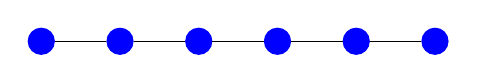
\begin{tikzpicture}
                \foreach \x in {0,...,5} {
                    \node[circle, draw=blue, fill=blue] (\x0) at (\x, 0) {};
                }

                \foreach \x [remember=\x as \lastx (initially 0)] in {1,...,5} {
                    \draw (\lastx0) to[] node[left]{}(\x0);
                }
            \end{tikzpicture}
            \\
            Diameter = $N-1$
        \end{center}
    \end{defi}

    \begin{defi}[Statisches Verbindungsnetzwerk]{Torus oder Ring}
        \begin{center}
            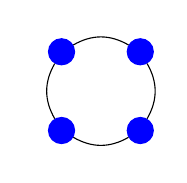
\begin{tikzpicture}
                \node[circle, draw=blue, fill=blue] (d0) at (0, 0) {};
                \node[circle, draw=blue, fill=blue] (d1) at (0, 1) {};
                \node[circle, draw=blue, fill=blue] (d2) at (1, 1) {};
                \node[circle, draw=blue, fill=blue] (d3) at (1, 0) {};
                \draw (d0) to[bend left] node[left]{}(d1);
                \draw (d1) to[bend left] node[left]{}(d2);
                \draw (d2) to[bend left] node[left]{}(d3);
                \draw (d3) to[bend left] node[left]{}(d0);
            \end{tikzpicture}
            \\
            Diameter = $\frac{N}{2}$
        \end{center}
    \end{defi}

    \begin{defi}[Statisches Verbindungsnetzwerk]{Torus}
        2D-Torus:
        \begin{center}
            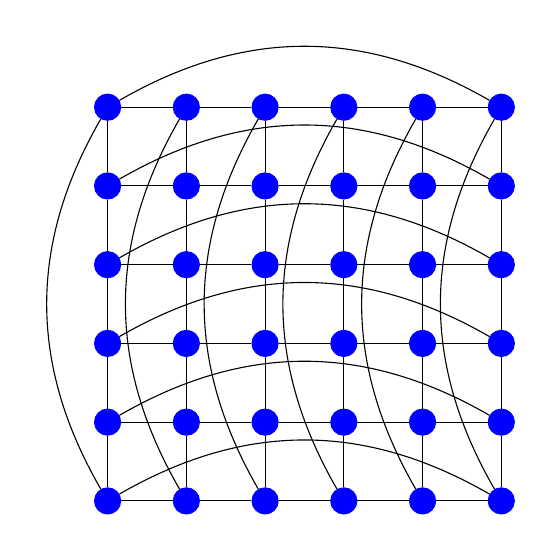
\begin{tikzpicture}[circlestyle/.style={circle, draw=blue, fill=blue}]
                \foreach \x in {0, ..., 5} {
                    \foreach \y in {0, ..., 5} {
                        \node[circlestyle] (\x\y) at (\x, \y) {};
                    }
                }

                \foreach \x in {0,...,5}{
                    \foreach \y [count=\yi] in {0,...,4}{
                        \draw (\x\y)--(\x\yi) (\y\x)--(\yi\x);
                    }
                }

                \foreach \x in {0,...,5} {
                    \draw (\x0) to[bend left] node[left]{}(\x5);
                }
                \foreach \y in {0,...,5}{
                    \draw (0\y) to[bend left] node[left]{}(5\y);
                }
            \end{tikzpicture}
            \\
            Diameter = $\sqrt{N}$
        \end{center}
    \end{defi}

    \begin{defi}[Statisches Verbindungsnetzwerk]{Gitter}
        2D-Gitter:\\
        \begin{center}
            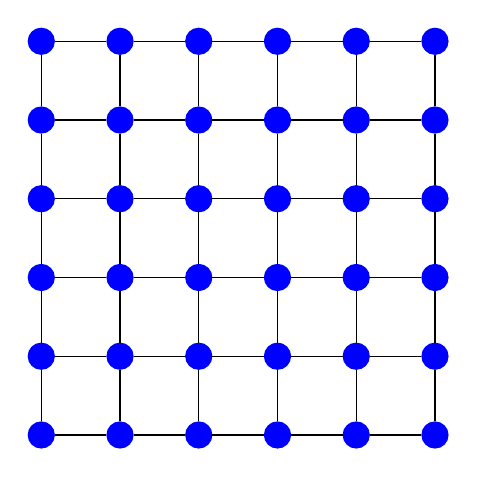
\begin{tikzpicture}[circlestyle/.style={circle, draw=blue, fill=blue}]
                \foreach \x in {0, ..., 5}{
                    \foreach \y in {0, ..., 5}{
                        \node[circlestyle] (\x\y) at (\x, \y) {};
                    }
                }

                \foreach \x in {0,...,5}{
                    \foreach \y [count=\yi] in {0,...,4}{
                        \draw (\x\y)--(\x\yi) (\y\x)--(\yi\x);
                    }
                }
            \end{tikzpicture}
            \\
            Diameter = $2\cdot\left(\sqrt{N} - 1\right)$
        \end{center}
    \end{defi}

    \begin{defi}[Statisches Verbindungsnetzwerk]{Hypercube}
        \begin{itemize}
            \item Anzahl der Knoten: $N = 2d$
            \item Diameter: $d = \log_2 N$
            \item Greycode Adressierung: Jeder Knoten verbunden mit $d$ anderen Knoten unterscheidet sich durch \emph{ein Bit} in der Adresse
            \item Beispiele: Intel iPSC und NCUBE
            \item Visualisierungen: \\
            \begin{tabular}{|c|c|c|c|}
                \hline
                
\begin{tikzpicture}[circlestyle/.style={circle, draw=blue, fill=blue}]
                    \node[circlestyle] (A) at (0,0) {};
                \end{tikzpicture} &
                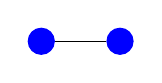
\begin{tikzpicture}[circlestyle/.style={circle, draw=blue, fill=blue}]
                    \node[circlestyle] (A) at (0,0) {};
                    \node[circlestyle] (B) at (1,0) {};
                    \draw (A) -- (B);
                \end{tikzpicture} &
                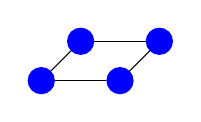
\begin{tikzpicture}[circlestyle/.style={circle, draw=blue, fill=blue}]
                    \node[circlestyle] (A) at (0,0) {};
                    \node[circlestyle] (B) at (1,0) {};
                    \draw (A) -- (B);

                    \node[circlestyle] (C) at (0.5, 0.5) {};
                    \node[circlestyle] (D) at (1.5, 0.5) {};
                    \draw (C) -- (D);

                    \draw (A) -- (C);
                    \draw (B) -- (D);
                \end{tikzpicture} &
                TODO: tikzpicture \\
                \hline
                0d & 1d & 2d & 4d \\
                \hline
            \end{tabular}
        \end{itemize}
    \end{defi}

    \begin{defi}[Statisches Verbindungsnetzwerk]{Baum}
        % TODO: https://de.wikipedia.org/wiki/Topologie_(Rechnernetz) (Quelle)
        \emph{Baum-Topologien} sind dadurch gekennzeichnet, dass sie eine Wurzel (der erste bzw. obere Knoten) haben, von der eine oder mehrere Kanten (Links) ausgehen.
        Diese führen weiterhin zu einem Blatt (Endknoten) oder \enquote{rekursiv} zu inneren Knoten von Teilbäumen.
        \begin{tabularx}{\textwidth}{|X|X|}
            \toprule
            Planares Layout: & Fetter Baum: (mehr Verbindungen erhöhen das Datenvolumen) \\
            \midrule
            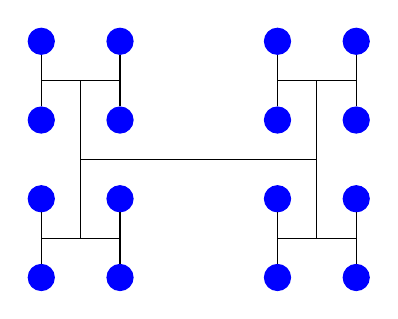
\begin{tikzpicture}[circlestyle/.style={circle, draw=blue, fill=blue}]
                \foreach \y in {0, ..., 3}{
                    \node[circlestyle] (0\y) at (0,\y) {};
                    \node[circlestyle] (1\y) at (1,\y) {};
                    \node[circlestyle] (3\y) at (3,\y) {};
                    \node[circlestyle] (4\y) at (4,\y) {};
                }
                % Connections between nodes
                \draw (00) -- (01);
                \draw (10) -- (11);
                \draw (30) -- (31);
                \draw (40) -- (41);

                \draw (02) -- (03);
                \draw (12) -- (13);
                \draw (32) -- (33);
                \draw (42) -- (43);
                %%%
                % Connections between connections
                \draw (0, 0.5) -- (1, 0.5);
                \draw (3, 0.5) -- (4, 0.5);

                \draw (0, 2.5) -- (1, 2.5);
                \draw (3, 2.5) -- (4, 2.5);

                \draw (0.5, 0.5) -- (0.5, 2.5);
                \draw (3.5, 0.5) -- (3.5, 2.5);

                \draw (0.5, 1.5) -- (3.5, 1.5);
                %%%
            \end{tikzpicture}
            &
            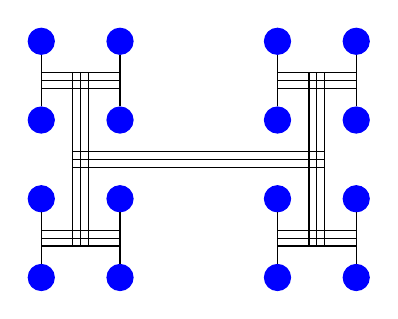
\begin{tikzpicture}[circlestyle/.style={circle, draw=blue, fill=blue}]
                \foreach \y in {0, ..., 3}{
                    \node[circlestyle] (0\y) at (0,\y) {};
                    \node[circlestyle] (1\y) at (1,\y) {};
                    \node[circlestyle] (3\y) at (3,\y) {};
                    \node[circlestyle] (4\y) at (4,\y) {};
                }
                % Connections between nodes
                \draw (00) -- (01);
                \draw (10) -- (11);
                \draw (30) -- (31);
                \draw (40) -- (41);

                \draw (02) -- (03);
                \draw (12) -- (13);
                \draw (32) -- (33);
                \draw (42) -- (43);
                %%%
                % Connections between connections
                \draw (0, 0.4) -- (1, 0.4);
                \draw (0, 0.5) -- (1, 0.5);
                \draw (0, 0.6) -- (1, 0.6);

                \draw (3, 0.4) -- (4, 0.4);
                \draw (3, 0.5) -- (4, 0.5);
                \draw (3, 0.6) -- (4, 0.6);

                \draw (0, 2.4) -- (1, 2.4);
                \draw (0, 2.5) -- (1, 2.5);
                \draw (0, 2.6) -- (1, 2.6);

                \draw (3, 2.4) -- (4, 2.4);
                \draw (3, 2.5) -- (4, 2.5);
                \draw (3, 2.6) -- (4, 2.6);

                \draw (0.4, 0.4) -- (0.4, 2.6);
                \draw (0.5, 0.4) -- (0.5, 2.6);
                \draw (0.6, 0.4) -- (0.6, 2.6);

                \draw (3.4, 0.4) -- (3.4, 2.6);
                \draw (3.5, 0.4) -- (3.5, 2.6);
                \draw (3.6, 0.4) -- (3.6, 2.6);

                \draw (0.4, 1.4) -- (3.6, 1.4);
                \draw (0.4, 1.5) -- (3.6, 1.5);
                \draw (0.4, 1.6) -- (3.6, 1.6);

                %%%
            \end{tikzpicture}
            \\
            \bottomrule
        \end{tabularx}
        \begin{center}
            Diameter = $\log_2 N$
        \end{center}
    \end{defi}

    \begin{bonus}{Übersicht statischer Verbindungsnetzwerke}
        \begin{tabularx}{\textwidth}{|l|X|X|X|}
            \toprule
            Topologie          & Anzahl der Verbindungskanäle pro Knoten & Maximale Entfernung (Diameter) & Gesamtanzahl der Verbindungskanäle \\
            \midrule
            Ring               & 2                                       & $\frac{N}{2}$                  & $N-1$                              \\
            \midrule
            Baum               & 3                                       & $2\cdot (\log_2 N - 1)$        & $N-1$                              \\
            \midrule
            2D - Gitter        & 4                                       & $2\cdot \sqrt{N}$              & $2\cdot N$                         \\
            \midrule
            3D - Gitter        & 6                                       & $3\cdot \sqrt[3]{N}$           & $3\cdot N$                         \\
            \midrule
            Hexagon. Gitter    & 6                                       & $3\cdot \sqrt[3]{N}$           & $3\cdot N$                         \\
            \midrule
            Hypercube          & $\log_2 N$                              & $\log_2 N$                     & $N \log_2 \frac{N}{2}$             \\
            \midrule
            Vollst. Vernetzung & $N - 1$                                 & 1                              & $N \cdot \frac{N-1}{2}$            \\
            \bottomrule
        \end{tabularx}
    \end{bonus}

    \subsubsection{Dynamische Verbindungsnetzwerke}

    \begin{defi}{Dynamisches Verbindungsnetzwerk}
        % TODO: https://de.wikipedia.org/wiki/Verbindungsnetzwerk (Quelle)
        \emph{Dynamische Verbindungsnetzwerke} zeichnen sich dadurch aus, dass die Verbindungen zwischen den Knoten über zum Netz gehörende Koppelelemente realisiert werden.

        Dabei können diese Koppelelemente in mehreren Stufen hintereinander angeordnet sein, weshalb man diese Art der Verbindungsnetzwerke nochmals in einstufige und mehrstufige Netze unterteilt.
        Eine Stufe enthält dabei eine gewisse Anzahl Koppelelemente.

        Genauer gesagt sorgt das Netz dafür, dass Senderknoten mittels einer Permutationsfunktion auf Empfängerknoten geschaltet werden.
        Dabei können entweder alle $n!$ Permutationen geschaltet werden, oder nur einige.
    \end{defi}

    \begin{defi}[Dynamisches Verbindungsnetzwerk]{Bus}
        % TODO: https://de.wikipedia.org/wiki/Verbindungsnetzwerk (Quelle)
        Bei einer \emph{Bus-Topologie} sind alle Geräte direkt mit demselben Übertragungsmedium, dem Bus verbunden.
        Es gibt keine aktiven Komponenten zwischen den Geräten und dem Medium.

        Durch die wahlweise Zuschaltung einzelner Verarbeitungsknoten zum Datentransfer an einen Bus ist das Bussystem eine typische dynamische Verbindungseinrichtung.

        Der Bus bildet die Engstelle im busgekoppelten Multiprozessorsystem, so dass auch Doppelbusse oder allgemein Mehrfachbusse eingesetzt werden.
    \end{defi}

    \begin{defi}{Crossbar}
        \begin{itemize}
            \item $M \times M$ Matrix
            \item einfaches Weiterleiten an mehrere Ausgänge
            \item komplexe Steuerung
            \item Verdrahtungsaufwand
            \item Pufferung bei Blockierungen
            \item Diameter = 1, d. h. beliebige Verbindungen können unter Einsatz jeweils nur einer Schaltzelle realisiert werden
        \end{itemize}
    \end{defi}

    \begin{defi}{Zellenbasierte Systeme}
        Zellen mit 2 Eingängen und 2 Ausgägen bilden die Basis für solche Systeme.
        \begin{itemize}
            \item 2 Bit $\to$ 4 Schaltzustände
            \item gerade Zellen
            \item kreuzende Zellen
            \item Eingänge mit mehreren Ausgängen verbunden (seltener genutzt)
        \end{itemize}
    \end{defi}

    \begin{defi}[Dynamisches Verbindungsnetzwerk]{Einstufiges Netzwerk}
        % TODO: https://de.wikipedia.org/wiki/Verbindungsnetzwerk (Quelle)
        \emph{Einstufige dynamische Verbindungsnetzwerke} bestehen aus nur einer so genannten Stufe von Schaltzellen beziehungsweise nur aus der Schaltzelle selbst.

        Die Zellen sind in der Regel eine mehr oder weniger komplexe Form eines Kreuzschienenverteilers (Crossbar), der selbst schon ein einstufiges dynamisches Verbindungsnetzwerk darstellt.

        TODO: Grafik
    \end{defi}

    \begin{defi}[Dynamisches Verbindungsnetzwerk]{Mehrstufiges Netzwerk}
        \emph{Mehrstufige dynamische Verbindungsnetzwerke} zeichnen sich dadurch aus, dass mehrere Stufen von Schaltzellen hintereinander geschaltet werden.
        Zwischen den Stufen besteht eine feste Verdrahtung.

        TODO: Grafik
    \end{defi}

    \begin{defi}{Omega-Netzwerk}
        \includegraphics[width=\textwidth]{images/OmegaNetwork.jpg}
        By Bjmyers17, CC BY-SA 3.0, \url{https://commons.wikimedia.org/w/index.php?curid=75639225}

    \end{defi}

    \begin{defi}[Dynamisches Verbindungsnetzwerk]{Zelle}
        % Die \emph{Zell-Topologie} kommt hauptsächlich bei drahtlosen Netzen zum Einsatz.

        % Eine Zelle ist der Bereich um eine Basisstation (z. B. Wireless Access Point), in dem eine Kommunikation zwischen den Endgeräten und der Basisstation möglich ist.
        % Innerhalb einer Zelle entspricht die Zell-Topologie der Bus-Topologie.
    \end{defi}

    \begin{defi}{Benes-Netzwerk}
        \includegraphics[width=\textwidth]{images/Benesnetwork.png}
        By Piggly - Own work, Public Domain, \url{https://commons.wikimedia.org/w/index.php?curid=2988080}
    \end{defi}

    \begin{defi}[Dynamisches Verbindungsnetzwerk]{Omega-Netzwerk}
        TODO
    \end{defi}

    \begin{defi}[Dynamisches Verbindungsnetzwerk]{Benes-Netzwerk}
        TODO
    \end{defi}

    \subsubsection{Cluster-Interconnects}

    \begin{defi}{Cluster-Interconnect}
        % TODO: https://de.wikipedia.org/wiki/Cluster_Interconnect (Quelle)
        Der \emph{Cluster-Interconnect} ist eine Verbindung zwischen den Cluster-Membern, über die alle Arten von relevanten Daten ausgetauscht werden.

        Sie wird in aller Regel als privates Netzwerksegment konzipiert, um höchstmögliche Betriebssicherheit zu gewährleisten oder auch andere Netzwerkarchitekturen abbilden zu können;
        denn diese Zwischenverbindung ist -- in Abhängigkeit von der Größe des Clusters -- mit möglichst geringer Latenz und hoher Übertragungsrate auszustatten, um keinen Flaschenhals zu schaffen.

        Dazu häufig verwendete Technologien sind Gigabit-Ethernet oder auch das teurere InfiniBand.
    \end{defi}

    \begin{defi}[Cluster-Interconnect]{InfiniBand}
        % TODO: https://de.wikipedia.org/wiki/InfiniBand (Quelle)
        \emph{InfiniBand} ist eine Spezifikation einer Hardwareschnittstelle zur seriellen Hochgeschwindigkeitsübertragung auf kurzen Distanzen mit geringer Latenz.

        Sie wird bevorzugt in Rechenzentren verwendet, beispielsweise für die Verbindungen der Server in Computerclustern untereinander und zur Verbindung zwischen Servern und benachbarten Massenspeichersystemen wie Storage Area Networks (SAN).

        InfiniBand benutzt bidirektionale Punkt-zu-Punkt-Verbindungen zur latenzarmen Datenübertragung mit Verzögerungszeiten unter \SI{2}{\micro\second}, und erreicht theoretische Datenübertragungsraten pro Kanal zwischen \SI{2,5}{\giga\bit\per\second} (SDR) und \SI{50}{\giga\bit\per\second} (HDR) in beide Richtungen.
        Bei InfiniBand können mehrere Kanäle zur Skalierung in einem Kabel transparent gebündelt werden.
    \end{defi}

    \begin{defi}[Cluster-Interconnect]{Gigabit Ethernet}
        Gigabit Ethernet \ldots
        \begin{itemize}[\ldots]
            \item wird vorwiegend in lokalen Netzwerken genutzt,
            auch für Heimanwender mit RJ45 Stecker für Kupferkabel (z.B. Lan-Buchsen am Router)
            \item ist für Glasfaser und (twisted-pair) Kupferkabel spezifiziert,
            höhrere Bandbreiten aber nur über Glasfaser umsetzbar: bis zu 100 Gb/s
            \item ist Switch-basiert und abwärtskompatibel
            \item nutzt spezielle Kollisionserkennung / -vermeidung,
            wie CSMA / CD (Carrier Sense Multiple Access with Collision Detection)
        \end{itemize}
    \end{defi}

    \begin{defi}[Verbindungsnetzwerk]{Klassifikation}
        \begin{center}
            \begin{forest}
                for tree={inner sep=2pt,outer sep=0pt,align=center,font=\sffamily\footnotesize,draw}
                [Verbindungsnetzwerk
                [statisch
                [ein-\\dimensional]
                [zwei-\\dimensional]
                [mehr-\\dimensional]
                ]
                [dynamisch
                [Bussysteme]
                [Zellenbasierte \\ Netze
                [einstufig]
                [mehrstufig
                [blockierend]
                [nicht-blockierend]
                ]
                ]
                [Kreuzschienenverteiler \\ (Crossbars)]
                ]
                ]
            \end{forest}
        \end{center}
    \end{defi}

    \subsection{Cache-Kohärenz}
    \begin{defi}{Cache-Kohärenz}
        \begin{itemize}
            \item wichtig bei Mehrprozessorsystemen mit Shared-Memory oder Shared Virtual Memory $\to$ SMP
            \item Maßnahmen zur Verhinderung von unterschiedlichen Versionen der gleichen Cache-Zeile in 2 oder mehreren Caches
            \item Technische Lösungen:
            \begin{itemize}
                \item \emph{Snooping Caches} (auf den Leitungen den Datenverkehr ausschnüffeln == to snoop) $\to$ Bus-basierte Systeme
                \item \emph{Directory-basierte Caches} $\to$ komplexere Verbindungsnetze
            \end{itemize}
        \end{itemize}
    \end{defi}

    \begin{defi}[Cache-Kohärenz]{Snooping Cache Protocols}
        Es gibt mehrere Snoopy-Protokolle (z.B. MESI).
        Sie basieren auf der \enquote{Invalidate}-Strategie:
        \begin{itemize}
            \item beim Schreiben von \enquote{shared data} wird ein \enquote{invalidate}-Signal an alle anderen Caches gesendet,
            die eine Kopie dieses Datums als ungültig kennzeichnen
            \item beim Lesen kann jeder Prozessor seine gültige Version der Cache-Zeile verwenden
            \item findet ein Prozessor beim Lesen kein gültiges Datum: Read-Miss
            \begin{itemize}
                \item bei \enquote{write-through}-Caches befindet sich das Memory immer im aktuellen Zustand:
                Datum wird in den anfordernden Cache gelesen
                \item bei \enquote{write-back}-Caches:
                suche (snoop) in den anderen Caches nach einer gültigen Version
            \end{itemize}
        \end{itemize}

        \begin{defi}[Cache-Kohärenz]{Directory-basierte Caches}
            Bus-basierte Snooping-Protokolle skalieren nicht bei großen Netzwerken mit NUMA-Architektur
            $\to$ Directory-Protokolle $\to$ ccNUMA \\
            Directory-basierte Protokolle sind ähnlich zu Snoopy-Protokoll.
            Das Directory hat ein Zustandsfeld mit 3 möglichen Zuständen:
            \begin{itemize}
                \item \emph{Shared:}     $\geq$ 1 Prozessor besitzen Daten, Memory aktuell
                \item \emph{Uncached:}   Kein Prozessor (kein Cache) besitzt gültige Daten
                \item \emph{Exclusive:}  1 Prozessor (owner) besitzt die Daten, Memory nicht aktuell
            \end{itemize}
        \end{defi}

        \subsection{Aufgaben}

        \begin{aufgabe}{Multiprozessoren}
            Nennen Sie zwei verschiedene Arten von nachrichtengekoppelten Multiprozessoren.
            \tcblower
            \begin{itemize}
                \item Massively Parallel Processor (MPP)
                \item Cluster Of Workstation (COW)
            \end{itemize}
        \end{aufgabe}

        \begin{aufgabe}{Multiprozessoren}
            Welche beiden Arten von speichergekoppelten Multiprozessor-Systemen wurden in der Vorlesung unterschieden?
            \tcblower
            \begin{itemize}
                \item Uniform Memory Access (UMA)
                \item Non Uniform Memory Access (NUMA)
            \end{itemize}
        \end{aufgabe}

        \begin{aufgabe}{Multiprozessoren}
            Zwischen welchen speichergekoppelten Multiprozessoren unterscheidet man je nach physikalischer Speicherorganisation?
            \tcblower
            \begin{itemize}
                \item Symmetric multiprocessor (SMP)
                \item Distributed shared memory Systeme
            \end{itemize}
        \end{aufgabe}

        \begin{aufgabe}{Distributed Memory Machines}
            Auf welche beiden Arten kann eine Distributed Memory Machine realisiert werden?
            \tcblower
            \begin{itemize}
                \item speichergekoppelt als shared virtual memory (SVM) $\to$ NUMA
                \item nachrichtengekoppelt (z.B. Cray T3E)
            \end{itemize}
        \end{aufgabe}

        \begin{aufgabe}{Verbindungsnetzwerk}
            Nennen und erklären Sie kurz die fünf grundlegenden Eigenschaften eines Verbindungsnetzwerkes.
            \tcblower
            \begin{tabularx}{\textwidth}{|X|X|}
                \toprule
                Eigenschaft            & Erklärung                                                                                                                                                    \\
                \midrule
                Latenz (latency)       & Zeit für den Transfer zwischen den Knoten                                                                                                                    \\
                \midrule
                Bandbreite (bandwidth) & $\frac{\text{transferierte Daten}}{Zeit}$, \newline Bandbreite eines Link: $\text{bw} = \omega \cdot \frac{1}{t} \left(\frac{\text{bit}}{\text{sec}}\right)$ \\
                \midrule
                Diameter               & maximale Distanz zwischen zwei beliebigen Prozessoren                                                                                                        \\
                \midrule
                Topologie              & wie sind die Nachbarknoten angeordnet und erreichbar                                                                                                         \\
                \midrule
                Statische oder \newline dynamische Leitungswege \\
                \bottomrule
            \end{tabularx}
        \end{aufgabe}

        \begin{aufgabe}{Verbindungsnetzwerk}
            Nennen Sie drei unterschiedliche Verbindungsnetzwerk-Topologien.
            \tcblower
            \begin{itemize}
                \item Torus
                \item (Hyper)cube / Mesh
                \item Tree / Fat Tree
            \end{itemize}
        \end{aufgabe}

        \begin{aufgabe}{Verbindungsnetzwerk}
            Durch welche physikalische Maßnahme kann bei einem Tree-Netzwerk der Durchsatz erhöht werden?
            \tcblower
            Man erstellt eine zunehmende Anzahl an Leitungen zur Wurzel hin ($\to$ Fat Tree).
        \end{aufgabe}

        \begin{aufgabe}{Verbindungsnetzwerk}
            Wie groß ist der Durchmesser eines 2D Torus mit N Gitterpunkten?
            \tcblower
            $$\sqrt{N}$$
        \end{aufgabe}

        \begin{aufgabe}{Verbindungsnetzwerk}
            Was sind die zwei gebräuchlichsten Netzwerktypen im HPC-Bereich?
            \tcblower
            \begin{itemize}
                \item Gbit Ethernet
                \item Infiniband
            \end{itemize}
        \end{aufgabe}

        \begin{aufgabe}{Cache-Kohärenz}
            Bei Mehrprozessorsystemen mit welchem Speicher ist Cache-Kohärenz wichtig?
            \tcblower
            \begin{itemize}
                \item Shared Memory
                \item Shared Virtual Memory
            \end{itemize}
        \end{aufgabe}

        \begin{aufgabe}{Cache-Kohärenz}
            Geben Sie zwei technische Lösungen an, um Cache-Kohärenz herzustellen.
            \tcblower
            \begin{itemize}
                \item Snooping Caches
                \item Directory-basierte Systeme
            \end{itemize}
        \end{aufgabe}

        \begin{aufgabe}{Cache-Kohärenz}
            Durch welches Hilfsmittel kann in Bus-basierten Systemen mit \enquote{write-back}-Caches Cache-Kohärenz realisiert werden?
            \tcblower
            Snoopy-Protokolle
        \end{aufgabe}

        \begin{aufgabe}{Cache-Kohärenz}
            Auf welcher Strategie basieren Snoopy-Protokolle?
            \tcblower
            Invalidate Strategie
        \end{aufgabe}

        \begin{aufgabe}{Cache-Kohärenz}
            Womit lässt sich Cache-Kohärenz bei Distributed Memory Systemen realisieren?
            \tcblower
            Directory basierte Protokolle
        \end{aufgabe}

        \begin{aufgabe}{Cache-Kohärenz}
            Wie lauten die drei möglichen Zustände des Zustandsfeldes der Directory bei einem Directory-basierten Protokoll?
            \tcblower
            \begin{itemize}
                \item Shared: $\geq$ 1 Prozessor besitzen Daten, Memory aktuell
                \item Uncached: Kein Prozessor (kein Cache) besitzt gültige Daten
                \item Exclusive: 1 Prozessor (owner) besitzt die Daten, Memory nicht aktuell
            \end{itemize}
        \end{aufgabe}